%-----------------------------------------------------------------------------
% Schriftgröße, Layout, Papierformat, Art des Dokumentes
%-----------------------------------------------------------------------------
\documentclass[12pt,					% Grundschriftgöße
							 oneside,			% einseitiges Dokument
							 a4paper,			% Papiergröße
							 halfparskip,		% Einzug bei einem Absatz
							 liststotoc,			% Verzeichniss (Abbildungen erc.) in das Inhaltverzeichnis
							 bibtotoc,			% Literaturverzeichnis ins Inhaltverzeichnis
							 fleqn,				% Mathematische Formeln linksbündig darstellen
							 pointlessnumbers]	% Punkt am Ende der Nummerierung des Inhaltsverzeichnisses entfernen
							 {scrreprt}

%-----------------------------------------------------------------------------
% Konstanten festlegen
%-----------------------------------------------------------------------------
\newcommand{\VerfasserA}{Nicole Goldmann}
\newcommand{\GeburtstagA}{20. August 1997}
\newcommand{\GeburtsortA}{Herbolzheim}
\newcommand{\VerfasserB}{Stefanie Weidemann}
\newcommand{\GeburtstagB}{25. August 1995}
\newcommand{\GeburtsortB}{Anklam}
\newcommand{\Titel}{Webapp für Studiende des Studienganges AIMMT}
\newcommand{\Betreuer}{Prof. Dr.-Ing. Herbert Litschke}
\newcommand{\blankpage}{
	\newpage
	\thispagestyle{empty}
	\mbox{}
	\newpage
}

%-----------------------------------------------------------------------------
% verwendete Pakete
%-----------------------------------------------------------------------------
\usepackage[T1]{fontenc}				% Wahl des Fonts, bzw. der Kodierung
\usepackage[utf8]{inputenc}			% Zeichkodierung , Umlaute erlauben
\usepackage[english,ngerman]{babel}		% neue deutsche Rechtschreibung verwenden
\usepackage{graphicx}					% erm�glicht das Einbinden von Grafiken, sehr wichtig!
\usepackage{fancyhdr}					% f�r formatierte Kopf- und Fu�zeilen
\usepackage{setspace}					% Package zum Kontrollieren von Leerr�umen
\usepackage{subfigure}					% erweiterte Darstellung von Bildern
\usepackage{listings}					% M�glickeit zum Anzeigen von Quelltexten
\usepackage{color,moreverb}				% Farben
\usepackage{lmodern}					% bietet neuere Schriften, sieht besser aus im Acrobat Reader
\usepackage{amsmath,amssymb}			% erweiteter Formelsatz und zus�tzliche Mathe-Symbole
\usepackage{booktabs}					% professionelle, typographisch richtige Tabellen
\usepackage{cite}						% f�r LibTex
%\usepackage{shortvrb}					% f�r Quellcode mit \begin{verbatim}
\usepackage[binary-units=true]{siunitx}	% Darstellung von Si-Einheiten
\usepackage{enumitem}					% custom itemiziation
\usepackage{textcomp}
\usepackage{url}
%-----------------------------------------------------------------------------
% Fu�notennummerierung nicht f�r jedes kapitel zur�cksetzen
%-----------------------------------------------------------------------------
\usepackage{chngcntr}
\counterwithout{footnote}{chapter}

%-----------------------------------------------------------------------------
% Einstellungen der Seitenr�nder
%-----------------------------------------------------------------------------
\usepackage[left=3cm,						% linker Rand
						right=3cm,			% rechter Rand
						top=1.5cm,			% oberer Rand
						bottom=1.5cm,		% unterer Rand
						includeheadfoot,	% bezieht die Kopf- und Fu�zeile mit ein
						bindingoffset=0cm]	% Bundsteg
						{geometry}

%-----------------------------------------------------------------------------
% Daten f�r die Titel des Artikels
%-----------------------------------------------------------------------------
\title{Semesterarbeit}
\author{\VerfasserA, VerfasserB}
\date{\today{}}

%-----------------------------------------------------------------------------
% Metadaten in pdf einf�gen
%-----------------------------------------------------------------------------
\usepackage[pdftex,
						pdfauthor={\VerfasserA, VerfasserA},					% Name des Autors
						pdftitle={\Titel},										% Name der Arbeit
						pdfcreator={MiKTeX, LaTeX with hyperref and KOMA-Script},	% Von was erzeugt
						%pdfsubject={Praktikumsbericht},							% Was f�r eine Arbeit ist es
						pdfkeywords={\Titel},
						plainpages=false,
						hypertexnames=false,
						pdfpagelabels]{hyperref}

%-----------------------------------------------------------------------------
% Schriftarten anpassen
%-----------------------------------------------------------------------------
\setkomafont{sectioning}{\rmfamily\bfseries}			% Titelzeilen
\setkomafont{caption}{\small}							% Schrift f�r Caption
\setkomafont{captionlabel}{\sffamily\bfseries\small}	% Schrift f�r 'Abbildung'
\setkomafont{chapterentry}{\small\bfseries}				% Schrift f�r Inhaltsverzeichnis
\setkomafont{chapter}{\large\bfseries}					% Schrift f�r Kapitel
\setkomafont{section}{\normalsize}						% Schrift f�r Section
\setkomafont{subsection}{\normalsize}					% Schrift f�r Subsection

%-----------------------------------------------------------------------------
% "Quellcode"-Unterschrift von Listing in Quellcode umbennen
%-----------------------------------------------------------------------------
\addto{\captionsngerman}{\renewcommand*{\lstlistingname}{Quellcode}}

%-----------------------------------------------------------------------------
% Farbe f�r Links in PDF-Dokumenten definieren
%-----------------------------------------------------------------------------
\definecolor{LinkColor}{rgb}{0,0,0}				% Festlegen einer neuen Farbe

\hypersetup{colorlinks=true,					% farbliche Links
						breaklinks=true,		% Zeilenumbruch erlauben
						linkcolor=black,		% Farbe f�r interne Links
						citecolor=black,		% Farbe f�r Links zum Literaturverzeichnis
						filecolor=LinkColor,	% Farbe f�r externe Dateilinks
						menucolor=LinkColor,	%
						urlcolor=LinkColor}		% Farbe f�r externe Links
						
%-----------------------------------------------------------------------------
% Definition f�r Quelltextlistings
%-----------------------------------------------------------------------------
\lstloadlanguages{C}

\definecolor{lbcolor}{gray}{0.95}			% Farbe f�r den Hintergrund definieren				
\definecolor{darkblue}{rgb}{0,0,.6}		% Farbe f�r Schl�sselw�rter
\definecolor{darkred}{rgb}{.6,0,0}		% Farbe f�r Strings
\definecolor{darkgreen}{rgb}{0,.6,0}		% Farbe f�r Kommentare

\lstset{language=C,								% Programmiersprache der Listings
				alsolanguage=Matlab,			% alternative Programmiersprache der Listings
				frame=none,								% keinen Rahmen
				frameround=ffff,					% wenn ein Rahmen dargestellt werden soll, sind die Ecken spitz
				captionpos=b,							% Position der Benennung
				numbers=left,							% Zeilennummern links angeben
				stepnumber=1,							% in welchem Abstand sollen Zeilennummern angeben werden (1 2 3..)
				numbersep=3pt,						% Abstand zwischen Nummerierung und Listing
				numberstyle=\tiny,				% gr�sse der Nummern
				breaklines=true,					% Zeilenumbruch zulassen
				breakautoindent=true,
				postbreak=\space,
				tabsize=4,								% Tabulator auf 4 setzen
				escapechar=\$,
				basicstyle=\scriptsize\ttfamily,
				keywordstyle=\color{darkblue}\bfseries\ttfamily,	% Darstellung der Schl�sselw�rter
				stringstyle=\ttfamily\color{darkred},  						% Darstellung der Strings
				commentstyle=\itshape\color{darkgreen},						% Darstellung der Kommentare
				showspaces=false,					% leerzeichen nicht anzeigen
				showstringspaces=false,		% keine Leerzeichen bei Strings anzeigen
				xleftmargin=.52cm,
				xrightmargin=.52cm,				
				backgroundcolor=\color{lbcolor}}	% Hintergrundfarbe des Listings
				
%-----------------------------------------------------------------------------
% Kopf- und Fusszeile bestimmen
%-----------------------------------------------------------------------------
\pagestyle{fancy}	
\fancyhf{}												% alle Felder l�schen
\fancypagestyle{plain}{}

% Kopfzeile rechts bzw. au�en
\fancyhead[R]{\nouppercase{\leftmark}}
% Linie oben
\renewcommand{\headrulewidth}{0.5pt}
% Fu�zeile rechts bzw. au�en
\fancyfoot[R]{\thepage}
%-----------------------------------------------------------------------------

%-----------------------------------------------------------------------------
% Begin des Dokuments
%-----------------------------------------------------------------------------
\begin{document} 						% Beginn des Dokumentes

	\renewcommand\lstlistingname{Code}
	\renewcommand\lstlistlistingname{Codeverzeichnis}
	
	%% Titel
	\begin{titlepage}
		\setlength\headsep{-5mm}
		\begin{figure}[!h]
			\begin{minipage}{0.8\textwidth}
				\textbf{Hochschule Wismar} \\
				University of Applied Sciences \\
				Technology, Business and Design \\
				Fakultät für Ingenieurwissenschaften, Bereich EuI \\
			\rule{\textwidth}{0.5pt}
			\end{minipage}
			\begin{minipage}[r]{0.1\textwidth}
				\begin{flushright}
					
\includegraphics[height=6\baselineskip]{pictures/HS-Wismar_Logo-FIW_2010-01.jpg}
				\end{flushright}
			\end{minipage}
		\end{figure}
		\vspace*{6cm}
		\begin{center}
			\Huge
			\textbf{Projektarbeit} \\
			\vspace{2cm}
			\large \Titel
			\begin{table*}[b]
				\begin{tabular}{rl}
					Gedruckt am: & \today \\
					\\
					von: & \VerfasserA \\
					& geboren am \GeburtstagA \\
					& in \GeburtsortA \\
					\\
					von: & \VerfasserB \\
					& geboren am \GeburtstagB \\
					& in \GeburtsortB \\
					\\
					Betreuer: & \Betreuer \\

				\end{tabular}
			\end{table*}
		\end{center}
	\end{titlepage}

	\onehalfspacing 					% 1 1/2-zeilig (package 'setspace')
	
	%\blankpage	%leeres Blatt zwischen Deckblatt und Inhaltsverzeichnis	
	%-----------------------------------------------------------------------------
	% Inhaltsverzeichnis
	%-----------------------------------------------------------------------------	
	\pdfbookmark[1]{Inhaltsverzeichnis}{toc}	% Inhaltsverzeichnis zu den Lesezeichen hinzufügen
	%\singlespacing 						% 1-zeilig
	\tableofcontents					% Inhaltverzeichnis einf�gen
	%\onehalfspacing 					% 1 1/2-zeilig (package 'setspace')

	%-----------------------------------------------------------------------------
	% Hauptteil
	%-----------------------------------------------------------------------------	
\newpage
\chapter*{Aufgabenstellung:}

\newpage

\chapter{Einleitung}

\chapter{Untersuchung der Hochschul Website}	
Studenten die Informationen zu ihrem Studiengang suchen brauchen teilweise sechs Klicks um von der Startseite der HS Wismar zur Semsterübersicht (AIMMT) zu gelangen. Innerhalb dieser Seiten gibt es einige Unstimmigkeiten und fehlerhaftes Fehlerhaftes Verhalten, welches im folgendem näher erläutert wird.
		\section{Analyse des Ist-Zustandes}
		Die Hochschulwebsite hat einen großen allgemeinen Teil der Informationen über die Hochschule enthält und hat Verlinkungen zu den drei Fakultätsseiten. Da die entwickelte Webanwendung für Studierende des Studiengangs Angewandte Informatik und Multimendiatechnik gedacht ist wird an dieser Stelle nur die Fakultätsseite der Ingenieurstechnik bzw. des Bereiches Elektrotechnik und Information.
		
		In der oberen Navigationsleiste gibt es nicht eindeutig erkennbare Icons für den Schnelleinstig und Informationen. Werden diese angeklickt, klappt sich ein Panel nach oben aus. Die obere Navigationsleiste ist nicht fixiert. Der Footer ist sehr groß und enthält teilweise die selben Verlinkungen wie in der Seitennavigation oben. Auf der Seite der Semsterübersicht gib es eine Akkordeonmenü welches nicht an allen Punkten anklickbar ist. Dieses Menü enthält ein Pfeil-Icon nach unten zeigend, welches dem User sugerriert das sich hinter dem Icon mehr Informationen enthalten.  Dieses Icon ist aber nicht anklickbar. Die Pfeil-Icons gibt es auf der gesamten Website als wiederkehrendes Symbol für Verlinkungen. Auf den Informationsseiten werden diese Icons allerdings auch als Auflistungszeichen verwendet. Weiterhin gibt es viel zu viele Querverweise. Beispielsweise auf einer Modulübersichtsseite gibt es Verlinkungen zu weiteren Studiengängen die dieses Modul besuchen, weitere Module die der/die Professor |in unterrichtet, die Forschungsthemen, Thesenthemen, und Jobs die der/die Professor|in anbietet. Diese Informationen gibt als sowohl auf der Modulübersicht als auch auf der persönlichen Seite der/des Professor|in. Der User wird überfordert, da zu viele Informationen gegeben werden. Desweiteren fehlt die Auflistung der Wahlpflichtmodule. Diese müssen umständlich im Modulhandbuch gesucht werden. 
		
		\section{Festlegung Systemanforderung}
		Die Hochschulwebsite ist sowohl für Studieninterssierte, als auch für eingeschriebene Studierende konzipiert. Um schneller an die wichtigsten Informationen zu gelangen, soll die Anwendung nur für eingeschriebene Studierende des Studiengangs Angewandte Informatik und Multimediatechnik dienen. Weiterhin sollen nur die wichtigsten Information kurz und knapp dargestellt werden. Daher hat jede Seite ein klares Ziel.	So ergeben sich weniger Verlinkungen, sodass der User immer genau weiß wo er sich befindet. Die heutigen Studierenden gehören zur Generation Smartphone. Daher soll der Ansatz "mobile first" verfolgt werden.
	

\chapter{Grundlagen}				
		\section{Technische Grundlagen}
				\subsection{Webcomponents}
				Web Components stellen eine Reihe von Webplattform-APIs dar. Mit Ihnen kann wiederverwendbares gekapseltes HTML erstellt und erweitert werden. Das HTML wird in Komponenten gegliedert die in jedem modernen Browser und jeder JavaScript-Bibliothek und jedem Framework verwendet werden kann. Web Components basieren auf vier Anforderungen: 
\begin{itemize}
\item \textit{Custom Elements:} Grundlage für das Erstellen neuer DOM-Elemente
\item \textit{Shadow Dom:} Definiert wie gekapseltes HTML in den Components verwendet wird
\item \textit{ES Modules:} Definiert die Einbindung und Wiederverwendung der JavaScript-Dateien
\item \textit{HTML Templates:} Definiert HTML-Fragmente die erst zur Laufzeit istanziiert werden
\end{itemize} Es existieren viel Bibliotheken mit denen die Erstellung von Web Components erleichtert wird, wie zum Beispiel Hybrids, LitElement, Polymer usw. Im folgenden wird die Bibliothek LitElement näher erläutert.\cite{webcom}
				\subsection{LitElement}
				LitElement ist eine Basisklasse zum Erstellen von Web Components. Sie verwendet lit-html um Templates zu definieren und zu rendern und fügt eine API zum Verwalten von Eigenschaften und Attributen hinzu.  Die Eigenschaften werden beobachtet und die Elemente werden asynchron aktualisiert, wenn sich ihre Eigenschaft ändert. 
					\subsubsection{Shadow-Dom}
					Der SHadow-Dom wird verwendet um den Template-Dom zu Kapseln. Er bietet drei wesentliche Vorteile: 
					\begin{itemize}
\item \textit{Dom-Scoping:} DOM-APIs finden keine Element im Schatten-Dom sodass globale Scripte keinen Zugriff haben
\item \textit{Style-Scoping:} gekapselte Styles haben keine Auswirkung auf den Rest des DOM-Baumes
\item \textit{Composition:} der Schatten-Dom der Komponente ist von untergeordneten Elementen getrennt, so kann gesteuert werden wie untergeordnete Elemente in das Template gerendert werden sollen\cite{webcom}
\end{itemize}
					
					\subsubsection{Templates}
					In einer Render-Funktion der Elementklasse wird das Template für die Component definiert. In dieser Funktion wird das rohe HTML in einem JavaScript template literal innerhalb von back-ticks geschrieben (siehe Abb. ). Die Render Methode kann alles zurückgeben was lit-html rendern kann. \cite{litelem}
					\begin{figure}[h]
						\centering
						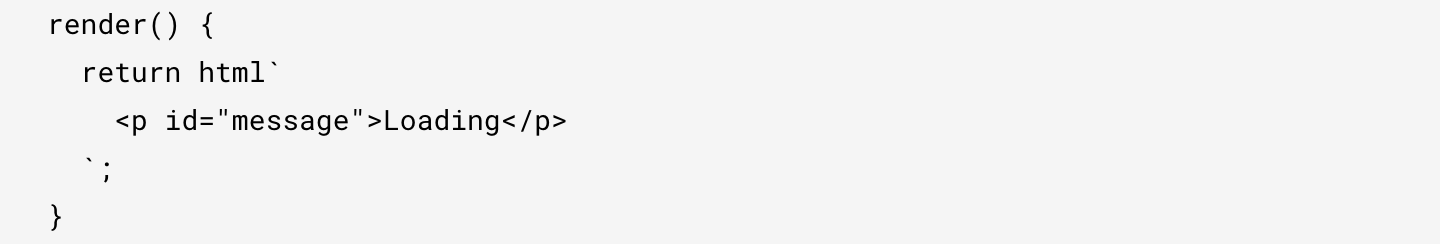
\includegraphics[width=1\textwidth]{pictures/render-function}
						\caption{Render-Funktion}\cite{litelem}
						\label{Render-Funktion}
					\end{figure}
				
					\subsubsection{Properties}
					LitElement verwaltet deklarierte Eigenschaften in einem statischen properties Getter, die entsprechenden Attribute werden in einem Elementkonstruktor initialisiert. So kann sicher gestellt werden das das bei einer geplanten Elementaktualiserung sich die deklarierte Eigenschaft ändert.  \cite{litelem}

					\subsection{Router}
Der Router übernimmt das Navigieren auf der gesamten Seite.
Er legt die angezeigte URL fest und managed welche HTML-Tags
(SPA's) dafür angezeigt werden.
Die verschiedenen Routen werden mit Namen und einem URL Pattern angelegt
und können auf diesem Wege auseinander gehalten werden.
Über Parameter und Querys können dann auch Informationen übertragen werden,
die für die neu aufgerufene Seite von belangen sind.

Wird nun ein Button mit einem Redirect auf eine neue SPA belegt,
registriert auch der Router den Klick und wechselt die 'route' Variable
auf den entsprechenden Namen, welcher zu der neuen URL zugehörig ist.
Anhand dieser Variable können alle nicht benötigten Seiten ausgeblendet
und die neue SPA angezeigt werden.

%		\section{Responsive Webentwicklung}	
%				\subsection{Positionierungseinheiten }
%					px, prozent, vh, vw, em, rem ...
%				\subsection{Umsetzung für verschiedene Displaygrößen}
%				\subsection{click- vs Touchevents}
%				\subsection{Elementanordnungen}
				


\chapter{Konzept}			
		\section{Use-Cases der Anwendung}	
		Das in Abbilding 4.1 gezeigte Use-Case-Diagram beinhalten zu Beginn zwei mögliche Interaktionen. Der User kann zwischen der Übersicht der Semester oder der Übersicht der Professoren und Mitarbeiter wählen. Wählt der User die Semester Übersicht kann er nun ein Semester wählen und bekommt anschließend die Module des jeweiligen Semesters angezeigt. Entscheidet er sich hier für ein Modul werden ihm die Details des Moduls gezeigt. In der Professoren und Mitarbeiter Übersicht kann der User eine Person auswählen und bekommt dann ebenfalls die Details zu dieser Person gezeigt.
\begin{figure}[h]
						\centering
						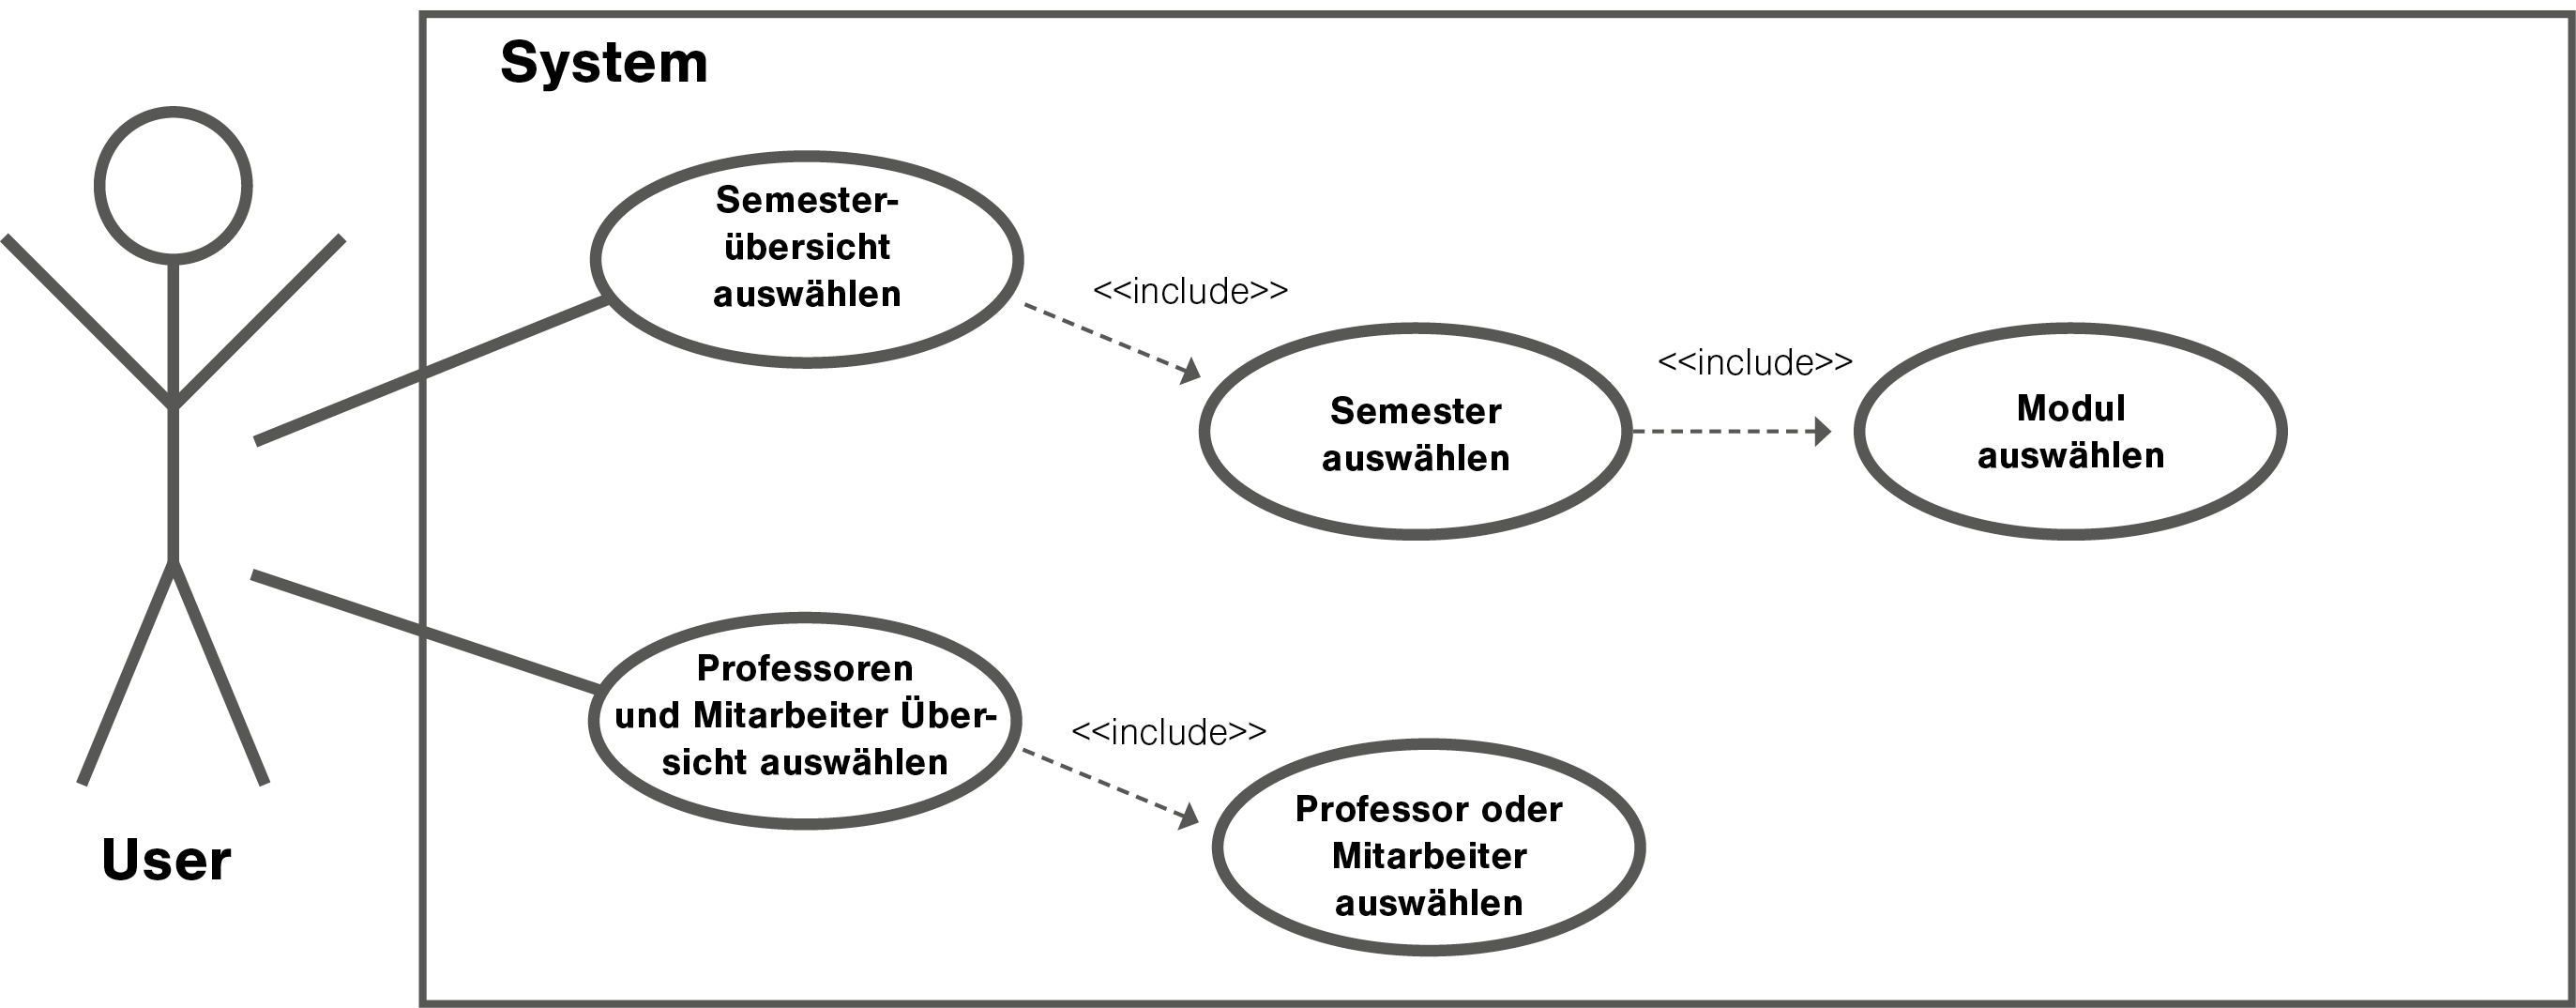
\includegraphics[width=1\textwidth]{pictures/use-cases.png}
						\caption{Use-Case-Diagramm (eigene Darstellung)}							
						\label{Use-Case-Diagramm}
					\end{figure}	
		
		\section{Systementwurf}
		Die Abbildung 4.2 zeigt die Zustände, in denen sich der User während der Benutzung der Anwendung befinden kann. Im Zustand der Startseite kann durch ein klick auf die gewünschte Übersicht zum einen in den Zustand der Semester Übersicht und zum andern in die Übersicht der Professoren und Mitarbeiter gewechselt werden. Diesen Zustandswechsel der beiden Übersichten kann jederzeit durch die untere Navigation getätigt werden. Im Zustand der Semester Übersicht kann durch ein klick auf ein Semester in den Zustand der Modul Übersicht gewechselt werden. Wählt der User hier durch ein klick ein Modul aus, wird die entsprechende Detailseite aufgerufen. Im Zustand der Professoren und Mitarbeiter Übersicht kann durch einen klick auf eine Person die entsprechende Detailseite der Person aufgerufen werden.
		
		
		\begin{figure}[h]
						\centering
						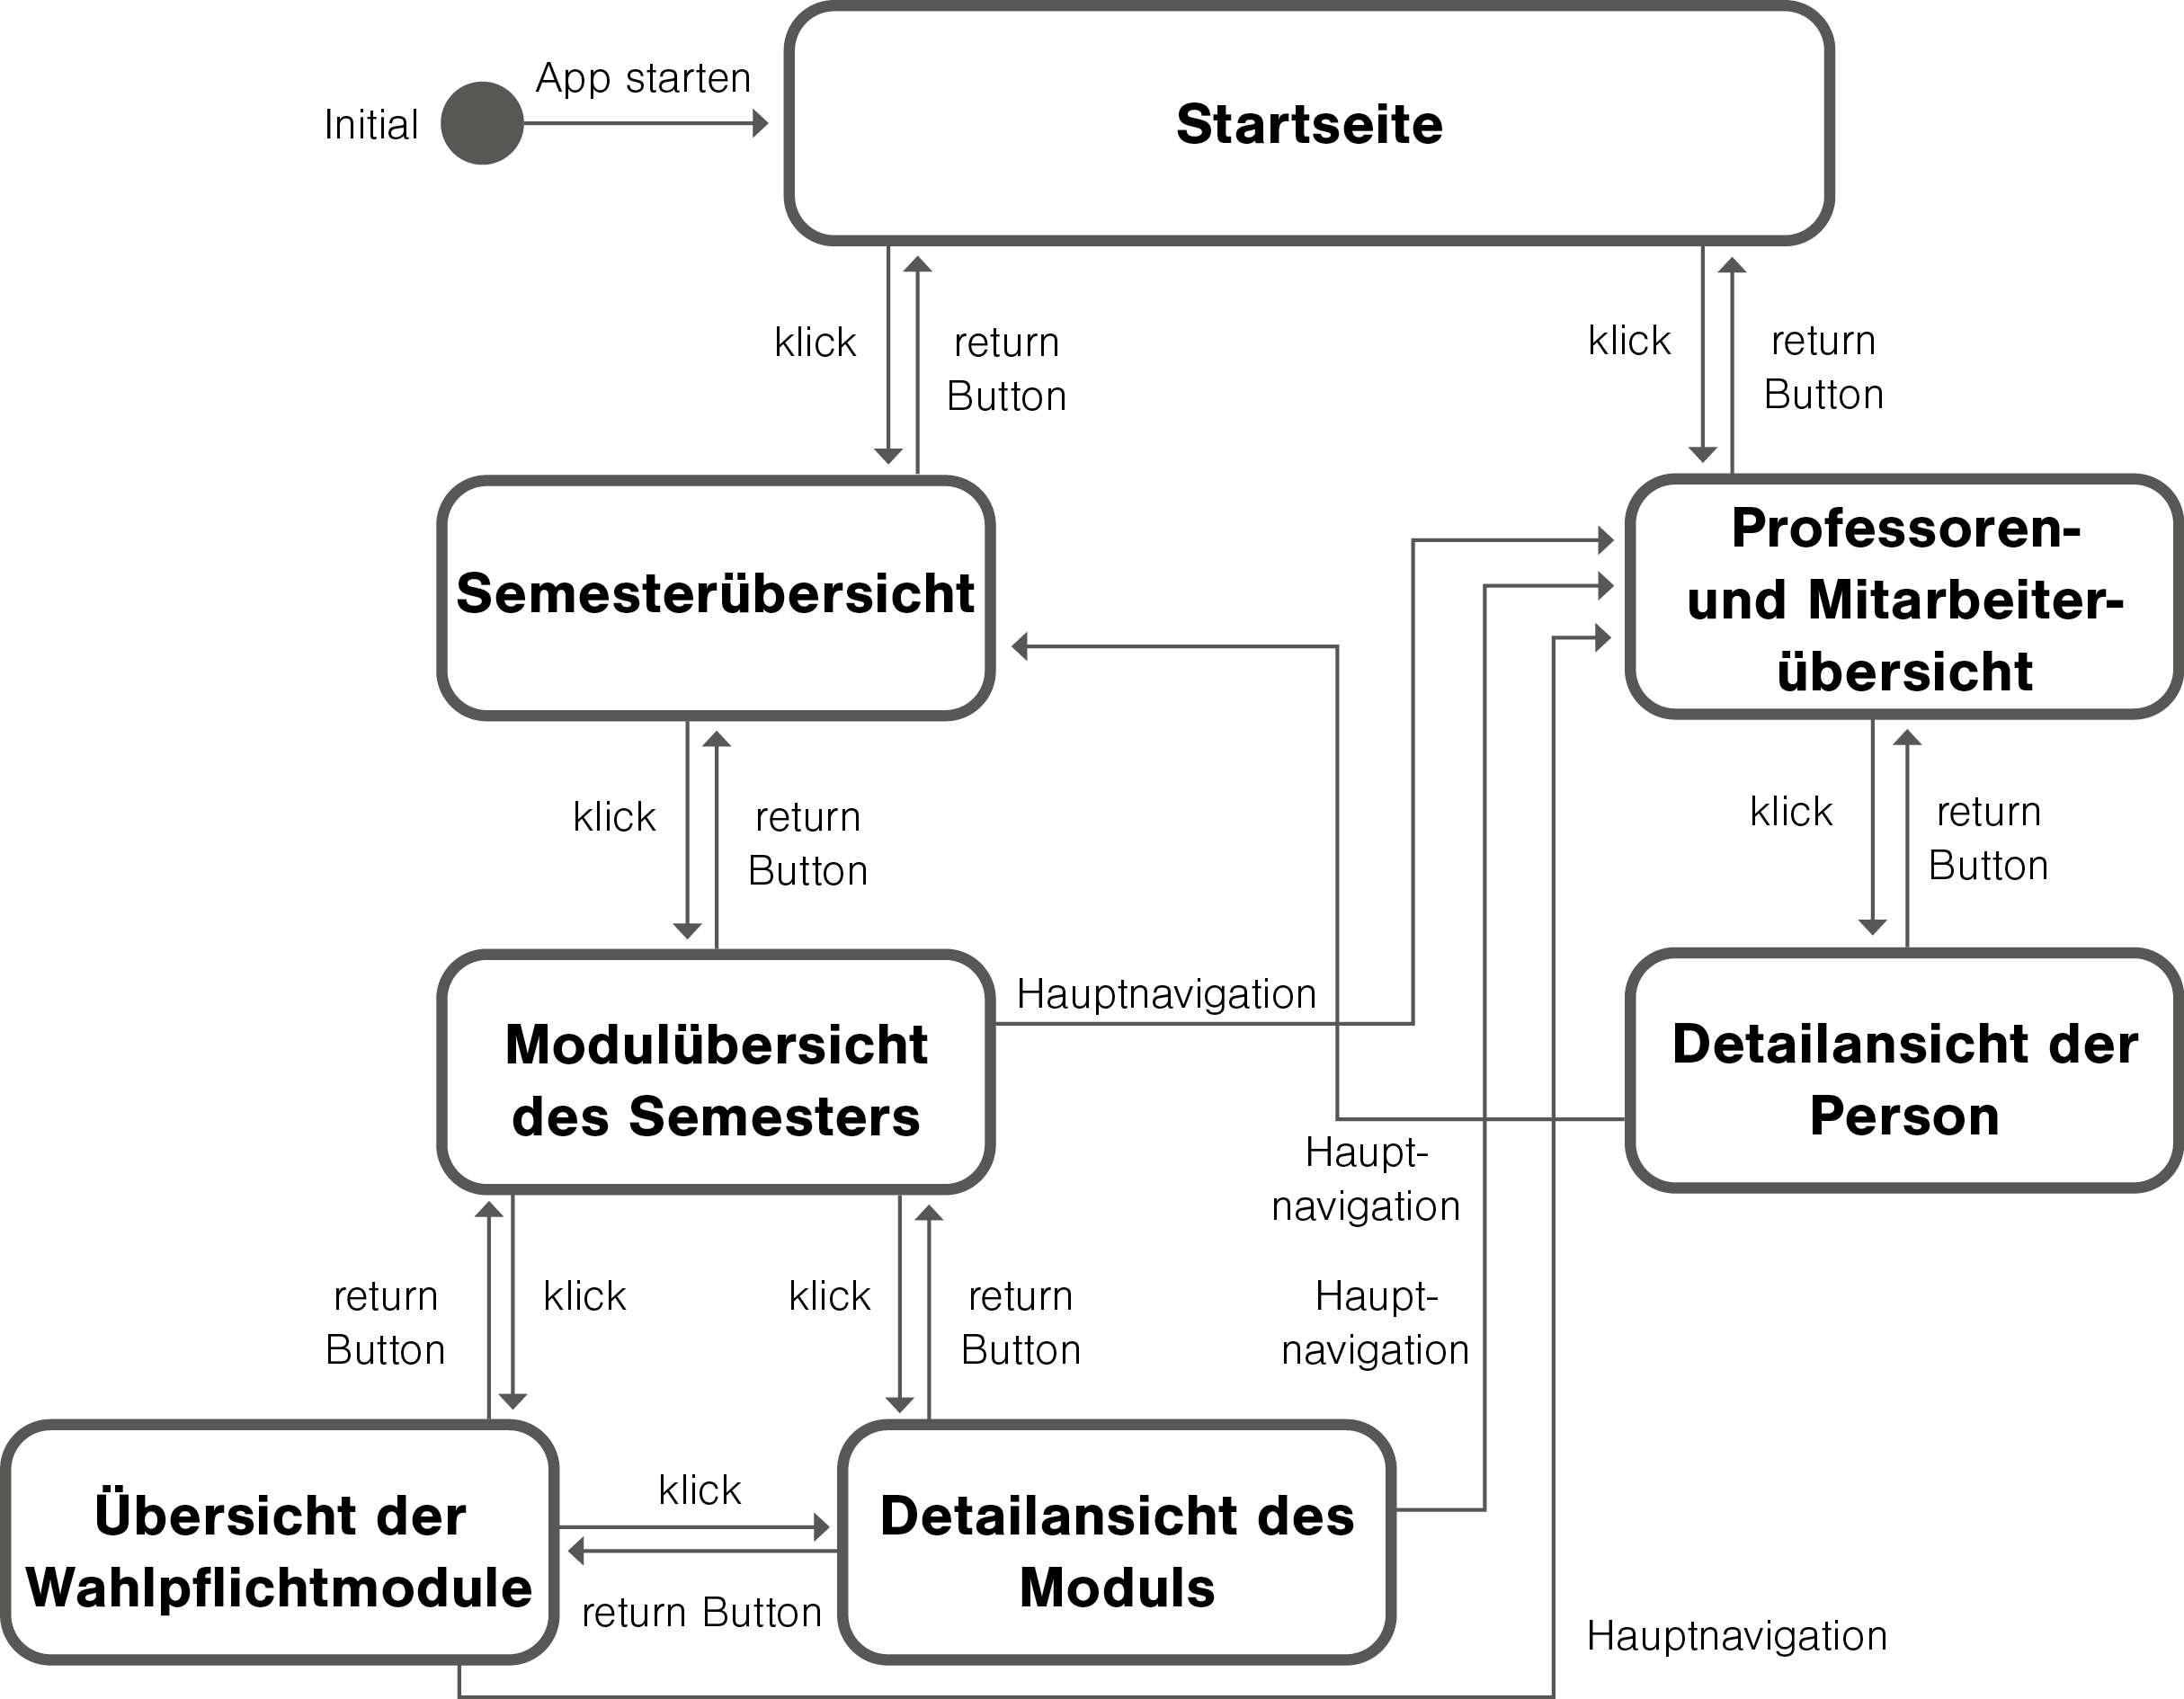
\includegraphics[width=0.7\textwidth]{pictures/zustandsdiagram.png}
						\caption{Zustandsdiagramm (eigene Darstellung)}						
						\label{Zustandsdiagramm}
					\end{figure}
		
\chapter{Implementierung}  

	\section{Components}
	\section{Router}



\chapter{Zusammenfassung und Ausblick}     


		
	
 	%-----------------------------------------------------------------------------
	% Literaturverzeichnis einfügen, 
	% Nutzung der BibTeX-Technologie --> literatur.bib 
	%-----------------------------------------------------------------------------
	
%	\bibliographystyle{unsrtdin}		%  Stil des Literaturverzeichnisses (hier nach DIN 1505)
%	\bibliography{literatur.bib}			% gibt Datei mit der Literatur an
	\nocite{*}						% damit alle in der DB enthaltende Einträge bearbeitet werden


\begin{thebibliography}{unsrt}
\bibitem{webcom} \textit{Introduction - What are web componts?} \\
https://www.webcomponents.org/introduction [17.05.2020]

\bibitem{litelem} \textit{LitElement} 2018 Polymer Project\\
https://lit-element.polymer-project.org/ [17.05.2020]

\bibitem{steamallg} \textit{Steam}, Valve Corporation\\
https://store.steampowered.com/about/ [19.05.2019]

\bibitem{steam} \textit{Steam Web API}, Valve Developer Community, 2019 \\
https://developer.valvesoftware.com/wiki/Steam\_Web\_API [17.05.2019]

\bibitem{neo4j} \textit{Eine Graphendatenbank für alle}, Michael Hunger, 2014, Entwickler.Press, ISBN: 978-3-86802-128-0

\bibitem{kommneo4j} \textit{Diese Vorteile bieten Graphdatenbanken}, Kommentar von Stefan Kolmar, 2017\\
https://www.bigdata-insider.de/diese-vorteile-bieten-graphdatenbanken-a-615118/ [17.05.2019]


\end{thebibliography}	

	%-----------------------------------------------------------------------------
	% Verzeichnisse
	%-----------------------------------------------------------------------------
	\listoffigures						% Bildverzeichnis einfügen
%	\listoftables						% Tabellenverzeichnis einfügen
%	\lstlistoflistings					% Quellcodeverzeichnis einfügen

	%-----------------------------------------------------------------------------
	% Anhang
	%-----------------------------------------------------------------------------	
	\appendix
	% Auch hier sind Gliederungen aller \chapter, \section
	

	%-----------------------------------------------------------------------------
	% Selbstständigkeitserklärung
	%-----------------------------------------------------------------------------	
	\chapter*{Selbstständigkeitserklärung}
	\addcontentsline{toc}{chapter}{Selbstständigkeitserklärung}
	\rhead{Selbstständigkeitserklärung} % rechts oben in der Kopfzeile Chapter darstellen
	Hiermit erklären wir, dass wir die hier vorliegende Arbeit selbstständig,
	ohne unerlaubte fremde Hilfe und nur unter Verwendung der aufgeführten
	Hilfsmittel angefertigt haben.

	\begin{tabular}{p{6cm}p{7cm}}
		\\
  		\\
  		\\
  		\\
  		Ort, Datum & Unterschriften
	\end{tabular}
	
	
	
\end{document}							% Ende des Dokuments
%-----------------------------------------------------------------------------
